\begin{figure}[htbp]
\centering
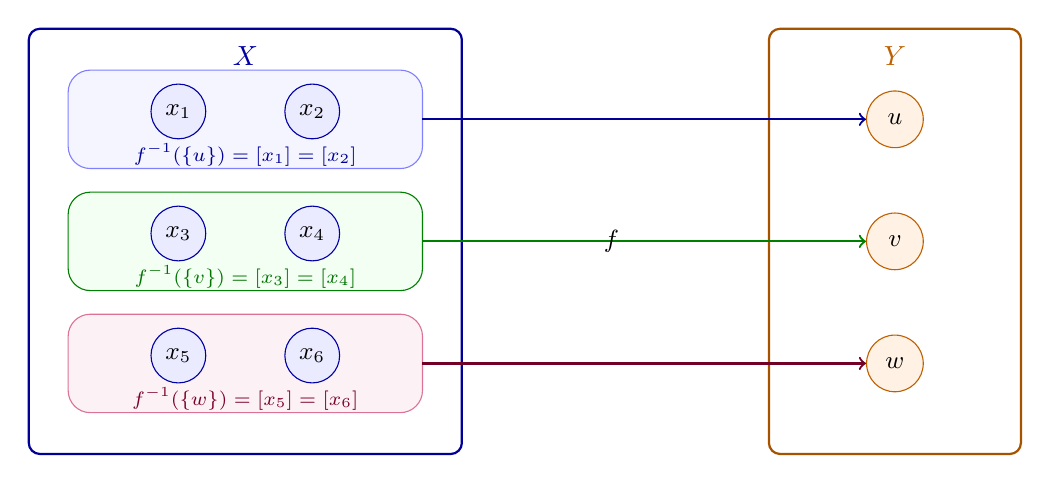
\begin{tikzpicture}[font=\small,element/.style={circle,draw=blue!65!black,fill=blue!8,minimum size=0.68cm},value/.style={circle,draw=orange!75!black,fill=orange!10,minimum size=0.72cm}]
    \draw[rounded corners,thick,draw=blue!60!black] (0,0) rectangle (5.5,5.4);
    \draw[rounded corners,thick,draw=orange!65!black] (9.4,0) rectangle (12.6,5.4);
    \node[font=\bfseries,text=blue!65!black] at (2.75,5.05) {$X$};
    \node[font=\bfseries,text=orange!75!black] at (11.0,5.05) {$Y$};
    \node[draw=blue!50,fill=blue!4,rounded corners=8pt,minimum width=4.5cm,minimum height=1.25cm] at (2.75,4.25) {};
    \node[draw=green!50!black,fill=green!5,rounded corners=8pt,minimum width=4.5cm,minimum height=1.25cm] at (2.75,2.7) {};
    \node[draw=purple!55,fill=purple!5,rounded corners=8pt,minimum width=4.5cm,minimum height=1.25cm] at (2.75,1.15) {};
    \node[element] at (1.9,4.35) {$x_1$};\node[element] at (3.6,4.35) {$x_2$};
    \node[element] at (1.9,2.8) {$x_3$};\node[element] at (3.6,2.8) {$x_4$};
    \node[element] at (1.9,1.25) {$x_5$};\node[element] at (3.6,1.25) {$x_6$};
    \node[font=\scriptsize,text=blue!60!black] at (2.75,3.8) {$f^{-1}(\{u\})=[x_1]=[x_2]$};
    \node[font=\scriptsize,text=green!45!black] at (2.75,2.25) {$f^{-1}(\{v\})=[x_3]=[x_4]$};
    \node[font=\scriptsize,text=purple!65!black] at (2.75,0.7) {$f^{-1}(\{w\})=[x_5]=[x_6]$};
    \node[value] (u) at (11.0,4.25) {$u$};
    \node[value] (v) at (11.0,2.7) {$v$};
    \node[value] (w) at (11.0,1.15) {$w$};
    \draw[->,thick,blue!60!black] (5.0,4.25) -- (u.west);
    \draw[->,thick,green!50!black] (5.0,2.7) -- (v.west);
    \draw[->,thick,purple!60!black] (5.0,1.15) -- (w.west);
    \node[font=\small\bfseries] at (7.4,2.7) {$f$};
\end{tikzpicture}
\caption{The relation $x\sim y$ defined by $f(x)=f(y)$ groups the domain into the fibers of $f$. Every element in a colored block has the same image, and each block is one equivalence class.}
\label{fig:function-fibers}
\end{figure}